%
% ======================================================================

\RequirePackage{docswitch}
% \flag is set by the user, through the makefile:
%    make note
%    make apj
% etc.
\setjournal{\flag}

\documentclass[\docopts]{\docclass}

% You could also define the document class directly
%\documentclass[]{emulateapj}

% Custom commands from LSST DESC, see texmf/styles/lsstdesc_macros.sty
\usepackage{lsstdesc_macros}
\usepackage{graphicx}
\graphicspath{{./}{./figures/}}
\bibliographystyle{apj}
% \usepackage{subcaption}
% \captionsetup{compatibility=false}
% Add your own macros here:
\usepackage{etoolbox}
%\usepackage{stackengine}
\setcounter{secnumdepth}{4}
\usepackage{csvsimple}
\usepackage{hyperref}
\usepackage{adjustbox}
\usepackage{xspace}
\usepackage{numprint}

\def\aapr{A\&A~Reviews}
\def\SLRealizer{\texttt{SLRealizer}\xspace}
\def\Object{\texttt{Object}\xspace}
\def\Source{\texttt{Source}\xspace}

% ======================================================================

\begin{document}

\title{\SLRealizer: LSST Catalog-level Realization of Gravitationally-lensed Quasars }

\maketitlepre

\begin{abstract}

The scale of the LSST dataset will be such that, when considering the
problem of finding lensed quasars, we should anticipate extracting as
much information out of the the catalogs as possible before turning to
the pixel-level data. In this work we explore the use of simple, low
multiplicity Gaussian mixture models for realizing gravitational lens
systems in LSST catalog space, to enable both large-scale data
emulation and fast initial lens-or-not classification. We demonstrate
the generation of toy \Source and \Object catalogs, and carry out a
simple machine learning classification using them.

\end{abstract}

% Keywords are ignored in the LSST DESC Note style:
\dockeys{methods: statistical, cosmology: gravitational lenses}

\maketitlepost

% ----------------------------------------------------------------------

\section{Introduction}
\label{sec:intro}

% The Large Synoptic Survey Telescope (LSST), a wide-field survey telescope with the diameter
% of 8.4m, will start running in Chile in 2020 \cite{LSST_overall}. This
% telescope has a 3.5 $deg$ of field of view, would cover around 30000
% $\textit{deg}^2$ in the sky, and uses $u$, $g$, $r$, $i$, $z$, and $y$
% filters \cite{LSSTScienceBookv2}. The telescope will give an extensive
% amount of astronomical data that could be used for the study of Solar
% System, Extragalactic structures, near-Earth asteroids, radiant radio
% sources, Dark Matter, and Dark Energy \cite{LSSTScienceBookv2}.

We anticipate being able to detect around 8000 strongly lensed quasar
systems, that will provide useful information on lens mass distributions
and cosmological time delay distances \citep{TM16,Twinkles}.
% Time delay could be used to infer cosmological parameters
% \cite{Treu2010} which describes the state of the universe.
Finding these lensed systems among the billions of objects detected and
measured by LSST \citep{LSSTScienceBookv2} is a key challenge.
Pixel-level searches \citep[e.g.\ ]{RINGFINDER} may be unfeasible,
unless the targets are efficiently pre-selected.  We can imagine doing
an initial lens classification on {\it catalog-level} data using machine
learning techniques, in order to make this pre-selection.

Machine learning to detect gravitational lensed systems is an active
area of research, with most of the focus to data being on galaxy-galaxy
``Einstein Ring'' systems, where  morphological classification using
Convolutional Neural Networks (CNN) should be effective
\citep{convolution_neural_network}. Early experiments show some
promising results \citep{LensExtractor,CMUDeepLens,Jacobs2017}. The LSST
catalog can be thought of as a database of pre-extracted image features,
which can be used as inputs to machine learning techniques. How much
lensing information do these features contain? How can we best train a
machine to classify the LSST \Object's as lenses or nots, without
requesting the images?

To answer these questions, we construct a mock LSST dataset, emulating
the action of the LSST data management software stack in generating the
data release catalog. Our simple emulator is called \SLRealizer: we
explain the assumptions it encodes in \autoref{sec:method} below. We
then carry out a simple demonstration machine classification, training
and testing the machine on a small toy \Object table, in
\autoref{sec:results}. We draw some conclusions about future work in
\autoref{sec:conclusions}.


\section{\SLRealizer}
\label{sec:method}

\subsection{Model assumptions}
\label{subsec:model}

\SLRealizer takes as input an extragalactic catalog of mock lensed
quasar systems, and emulates the LSST data release catalog measurements
of those lenses. It's assumptions are that the \Object's and \Source's
in the catalog tables can be simply represented as mixtures of
Gaussians, and measurements of them derived from those Gaussian
mixtures.

Specifically, we assume that a lensed quasar system is composed of 2 or
4 point-like sources (for doubles and quads respectively), plus a lens
galaxy that can be represented with an elliptically-symmetric Gaussian
surface brightness distribution. The seeing FWHM in each visit is used
to define a circularly-symmetric Gaussian PSF.

\SLRealizer models the action of the LSST DM stack deblender as
returning a single \Object for each galaxy-scale lensed quasar system.
Its ``null deblender'' yields predictions of the flux, position, size
and ellipticity of each measured \Source calculated by realizing the
surface brightness of the PSF-convolved system on a pixelated
``pseudo-image'' grid, and then numerically integrating this image to
obtain its zeroth, first and second moments. We use the python \GalSim
package to carry out the pseudo-image manipulations, and choose a pixel
scale of 0.2~arcseconds (the same as the LSST detectors).

In future, Gaussian noise will be added to each measurement.

The \Object table is then emulated by simply averaging the available
\Source flux, position, size and ellipticity measurements in each
filter.


\subsection{Emulator Inputs}
\label{subsec:inputs}

Twinkles, a simulated LSST sky with observed with six filters for ten
years, used ten years of mock observation history from the LSST
Project's baseline cadence simulation, \texttt{minion\_1016}. We use
this history file to define an MJD date, filter, seeing FWHM and 5-sigma
limiting depth for each visit in the history, and select just the first
three years of observations, which yields 263 observation epochs.

\begin{table}[!h]
\csvautotabular{../../data/twinkles_observation_history_head.csv}
%https://texblog.org/2012/05/30/generate-latex-tables-from-csv-files-excel/ %bug
% PJM: The following doesn't work:
% \csvreader[head to column names, tabular=lllll,
% table head=\toprule, \bfseries obsHistID & \bfseries expMJD & \bfseries filter & \bfseries FHWMeff & \bfseries fiveSigmaDepth \\ \midrule,
% table foot=\bottomrule,
% filter test=\ifnumless{\obshistid}{187546}]%
% {../../data/twinkles_observation_history.csv}{}{%
% \thecsvrow & \obshistid & \expmjd & \filter & \fwhmeff & \fiveSigmaDepth }
%
\caption{A few entries of the Twinkles mock observation history data.
The full dataset can be accessed
\href{https://github.com/LSSTDESC/SLRealizer/blob/master/data/twinkles_observation_history.csv}{here}.}
\end{table}

We use the OM10 mock lens catalog \citep{OM10} to define the properties
of the lens galaxy and lensed quasar images. We selected LSST-like
systems by querying with magnitude cut of 22.5. Colors were computed
using the \texttt{OM10} package, which makes use of the \texttt{lenspop}
code \citep{lenspop} for estimating galaxy and quasar colors.

\begin{figure}
    \centering
    \begin{minipage}{0.48\linewidth}
        \centering
        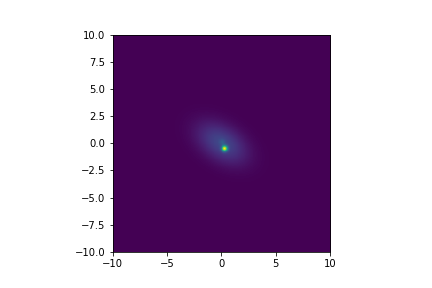
\includegraphics[width=\linewidth]{beforenulldeblend.png}
    \end{minipage}\hfill
    \begin{minipage}{0.48\linewidth}
        \centering
        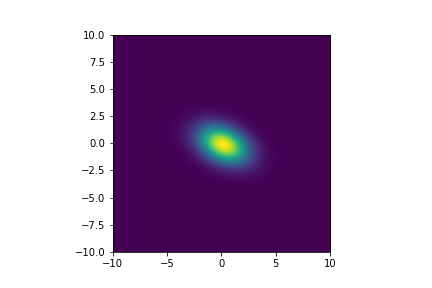
\includegraphics[width=\linewidth]{afternulldeblend.png}
    \end{minipage}
    \caption{Example null-deblending in OM10 lens system 4898214. Image
    axes show offsets from the  center of the lensed system in arcsec.
    Left: Realization of the lens system with zero-width PSF. The
    brightest source is the lensing galaxy, and there are two dimmer
    quasar images near the galaxy. There is only one quasar image that
    is obvious; this makes the blended object appear elliptical. Right:
    Realization of the lens system with realistic PSF. All the
    components of the system appear blended together. The color bar
    shows rescaled surface brightness: overall, flux is conserved
    between the two images.}
    \label{fig:null-deblend}
\end{figure}

% ----------------------------------------------------------------------

\section{Toy Emulated LSST Data}
\label{sec:data}

A snippet from our toy \Source catalog is shown below, in
\autoref{tab:source}. As you can see, for now we have not added error
terms, nor calculated the positions (RA and DEC).

\autoref{tab:object} shows an excerpt from our toy \Object catalog.


%%%%%%%%%%%%%%%%%%%%%%%%%%%%%%%%%%%%%%%%%%%
\begin{table}[!h]
\centering
\begin{tabular}{|l|l|l|l|l|l|l|l|l|l|l|}
\hline
lensid   & MJD          & filter & RA & RA\_err & DEC & DEC\_err & x              & x\_com\_err & y               & y\_com\_err \\ \hline
710960   & 59823.286523 & g      & 0  & 0       & 0   & 0        & 2.1350  & 0           & 1.2151 & 0			\\
17432684 & 59823.286523 & g      & 0  & 0       & 0   & 0        & 0.1226 & 0           & 0.7593  & 0           \\
50310149 & 59823.286523 & g      & 0  & 0       & 0   & 0        & 0.2527 & 0           & 0.4665  & 0           \\
52812164 & 59823.286523 & g      & 0  & 0       & 0   & 0        & 0.3874 & 0           & -0.3413 & 0          \\ \hline
\end{tabular}
\begin{tabular}{|l|l|l|l|l|l|l|l|l|l|}
\hline
flux          & flux\_err       & size          & size\_err & e1               & e2                & e               & phi             & psf\_sigma & sky       \\ \hline
21.9127 & 0.03549 & 1.4501 & 0         & 0.2386    & 0.3360    & 0.4121  & 0.4766  & 1.093153   & 24.377204 \\
18.2072 & 0.03549& 1.1802  & 0         & -0.0550 & -0.004712  & 0.05525 & 0.04270 & 1.093153   & 24.377204 \\
5.9831 & 0.03549 & 1.2253 & 0         & -0.05931 & 0.02588     & 0.06471 & -0.2057 & 1.093153   & 24.377204 \\
6.2727 & 0.03549 & 1.2102  & 0         & -0.03114 & -0.05654  & 0.06455 & 0.5336  & 1.093153   & 24.377204 \\ \hline
\end{tabular}
\caption{A few sample entrees of the toy \Source catalog. The full toy object catalog can be viewed \href{https://www.dropbox.com/s/muqui8eu3kxox2l/toy_source_catalog.csv?dl=0}{here}}
\label{tab:source}
\end{table}
%%%%%%%%%%%%%%%%%%%%%%%%%%%%%%%%%%%%%%%%%%%



%%%%%%%%%%%%%%%%%%%%%%%%%%%%%%%%%%%%%%%%%%%
\begin{table}[!h]
\centering

\begin{tabular}{|l|l|l|l|l|l|l|l|l|l|l|l|l|}
\hline
lensid     & u\_flux & u\_x   & u\_y   & u\_size & u\_flux\_err & u\_x\_com\_err & u\_y\_com\_err & u\_size\_err & u\_e1   & u\_e2   & u\_e   & u\_phi \\ \hline
710960.0   & 37.0846 & 2.2817 & 1.2996 & 1.4151  & 0.2511       & 0.0            & 0.0            & 0.0          & 0.1399  & 0.205   & 0.2496 & 0.4574 \\ \hline
17432684.0 & 26.7018 & 0.1211 & 0.7633 & 0.971   & 0.2516       & 0.0            & 0.0            & 0.0          & -0.0968 & -0.0092 & 0.0972 & 0.0497 \\ \hline
\end{tabular}

\begin{tabular}{|l|l|l|l|l|l|l|l|l|l|ll|}
\hline
g\_flux & g\_x   & g\_y   & g\_size & g\_flux\_err & g\_x\_com\_err & g\_y\_com\_err & g\_size\_err & g\_e1   & g\_e2   & g\_e   & g\_phi	\\ \hline
19.9485 & 2.1555 & 1.2328 & 1.4608  & 0.1244       & 0.0            & 0.0            & 0.0          & 0.1967  & 0.2768  & 0.3395 & 0.4765 \\ \hline
17.5991 & 0.1221 & 0.7518 & 1.2413  & 0.1244       & 0.0            & 0.0            & 0.0          & -0.0532 & -0.0045 & 0.0534	& 0.0425	\\ \hline
\end{tabular}


\begin{tabular}{|l|l|l|l|l|l|l|l|l|l|l|l|}
\hline
r\_flux & r\_x   & r\_y   & r\_size & r\_flux\_err & r\_x\_com\_err & r\_y\_com\_err & r\_size\_err & r\_e1   & r\_e2   & r\_e   & r\_phi \\ \hline
31.0886 & 2.27   & 1.2928 & 1.2608  & 0.0923       & 0.0            & 0.0            & 0.0          & 0.1693  & 0.2395  & 0.2933 & 0.4779 \\
25.2258 & 0.1215 & 0.7617 & 0.9958  & 0.0923       & 0.0            & 0.0            & 0.0          & -0.0867 & -0.0078 & 0.087  & 0.0457 \\ \hline
\end{tabular}

\begin{tabular}{|l|l|l|l|l|l|l|l|l|l|l|l|}
\hline
i\_flux & i\_x   & i\_y   & i\_size & i\_flux\_err & i\_x\_com\_err & i\_y\_com\_err & i\_size\_err & i\_e1   & i\_e2   & i\_e   & i\_phi \\ \hline
26.2547 & 2.3012 & 1.3075 & 1.2154  & 0.0433       & 0.0            & 0.0            & 0.0          & 0.1521  & 0.2146  & 0.263  & 0.4773 \\
22.747  & 0.1217 & 0.7612 & 1.0063  & 0.0433       & 0.0            & 0.0            & 0.0          & -0.0813 & -0.0071 & 0.0816 & 0.0436 \\ \hline
\end{tabular}

\begin{tabular}{|l|l|l|l|l|l|l|l|l|l|l|l|}
\hline
z\_flux & z\_x   & z\_y   & z\_size & z\_flux\_err & z\_x\_com\_err & z\_y\_com\_err & z\_size\_err & z\_e1   & z\_e2   & z\_e   & z\_phi \\ \hline
19.7955 & 2.264  & 1.2879 & 1.2545  & 0.0322       & 0.0            & 0.0            & 0.0          & 0.1595  & 0.2247  & 0.2755 & 0.4767 \\
18.0387 & 0.1216 & 0.7587 & 1.0622  & 0.0315       & 0.0            & 0.0            & 0.0          & -0.0751 & -0.0064 & 0.0754 & 0.0426 \\ \hline
\end{tabular}

\caption{A few sample entries of our toy \Object catalog. The full toy
object catalog can be viewed
\href{https://www.dropbox.com/s/ob51rxjexzuervl/toy_object_catalog.csv?dl=0}{here}}
\label{tab:object}
\end{table}
%%%%%%%%%%%%%%%%%%%%%%%%%%%%%%%%%%%%%%%%%%%


% ----------------------------------------------------------------------

\subsection{Feature Selection}
\label{subsec:feature}

For now, we focused on classifying the lensed systems from the SDSS
galaxies. We expect the lensed images to appear near the bright, massive
galaxies. Thus, if we can differentiate the galaxies with lensed images
with the galaxies without them, it would be really helpful.

We expect that the quasar images will be brighter in the shorter
wavelength filters. The galaxies will be brighter in the longer
wavelength filters. Thus, when we observe a lensed system through a $u$
filter (the shortest wavelength filter that OM10 has), we will see the
more stretched object because of the contribution from the quasar
images. However, in the $z$ band, we will see a round object because of
the contribution from the lens. By comparing the features in the $u$
filter and the $z$ filter, we will thus be able to see bigger changes in
the properties for the lensed systems than SDSS galaxies.

The features that we could get from the object table is changes in the
first moment along the x-axis (reference to the $r$ filter), changes in
the first moment along the y-axis (reference to the $r$ filter), changes
in the position (reference to the $r$ filter), ellipticities, rotation
angles, fluxes, and sizes.

The catalog of SDSS galaxies also provides the same features. Magnitude
systems are the same in both SDSS and OM10, and the units are scaled to
be the same. However, the only difference was in the sizes. SDSS's
definition of size was $I_{xx}$ + $I_{yy}$. Galsim calculates the size
of OM10 systems by calculating the determinant of the second moment
($M=I_{xx}I_{yy}-I_{xy}I_{xy}$) and applying the fourth root on it
($\sqrt[4]{M}$). In order to solve the problem by scaling the SDSS
sizes, we multiplied the power of pixel-to-arcsec ratio to change the
unit to arcseconds, multiplied two to convert the half size to the full
size, and applied the square root to the value to get a right dimension.

Using these values, we computed various additional features. We plotted
SDSS galaxies and OM10 lensed systems onto the corner plot
\autoref{subsec:feature}, and chose the features that differentiated
OM10 lensed systems from SDSS galaxies the most.

\subsection{Classification}
\label{subsec:classification}

We have 2323 OM10 lensed systems and 16000 SDSS galaxies. In order to
make the balanced test data set, we randomly selected 2323 SDSS
galaxies. We mixed the order of those two samples so that there will be
a roughly same number of each OM10 and SDSS samples in both the test and
the training data. Then, using the scikit train$\_$test$\_$split method,
we selected 75$\%$ of the data to be the training set and performed the
test on the remaining 25$\%$.

According to the \texttt{scikit-learn}'s
\href{http://scikit-learn.org/stable/tutorial/machine_learning_map/index.html}
{flowchart for choosing the right estimator}, we were able to choose
three different algorithms for the classification purposes. We did have
more than 50 samples, we were predicting a category, we did have a
labeled data, and we had less than 100K samples in a text data. This
yields Linear SVC, KNeighbors Classifier, and Ensemble classifiers such
as Random Forest.

Detailed results are in \autoref{subsec:classification_data}.









\subsection{Feature Selection}
\label{subsec:feature_data}

Full corner plots can be viewed in the
\href{https://github.com/jennykim1016/SLRealizer/blob/master/notebooks/SDSSvsOM10.ipynb}{SLRealizer's
GitHub repository's notebook folder}.

As mentioned in \autoref{subsec:feature}, we thought comparing features
between $u$ and $z$ filter will be discriminatory. We chose six main
features that we thought would change dramatically between the filters
for OM10 lenses -- sizes, ellipticities (e), rotation angles of galaxies
($\phi$), magnitudes, positions($\Delta$ x), and the angle between
ellipticity vector and the rotation vector ($\omega = \frac{e \cdot
\phi}{ \left | e \right | \left | \phi \right |}$).

\begin{figure}
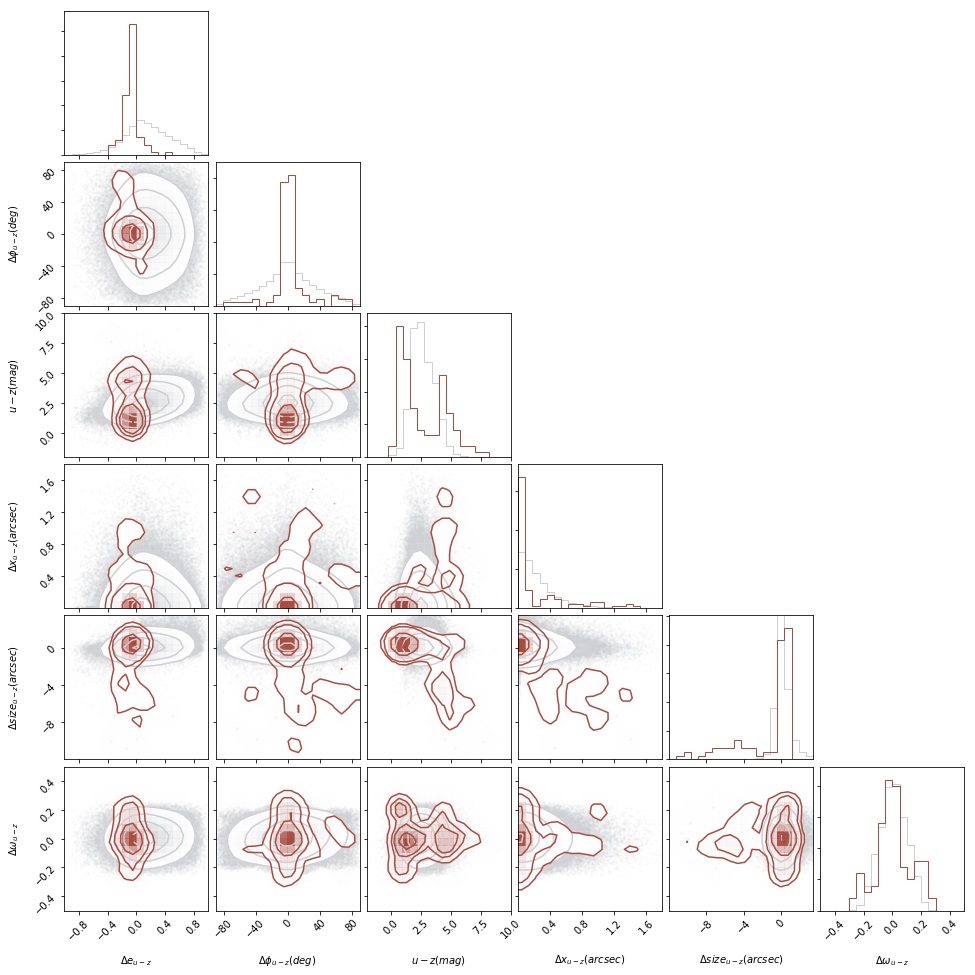
\includegraphics[width=0.9\columnwidth]{cornerplot.png}
\caption{The cornerplot with six features.}
 \label{fig:cornerplot}
\end{figure}

Here, the centroid of the yellow points(SDSS galaxies) and the purple
points(OM10 systems) differed the most for size. Still, we could
quantify the importance of the features by putting all the data into the
Random Forest Algorithms. The results were as follows.

\begin{figure}[!h]
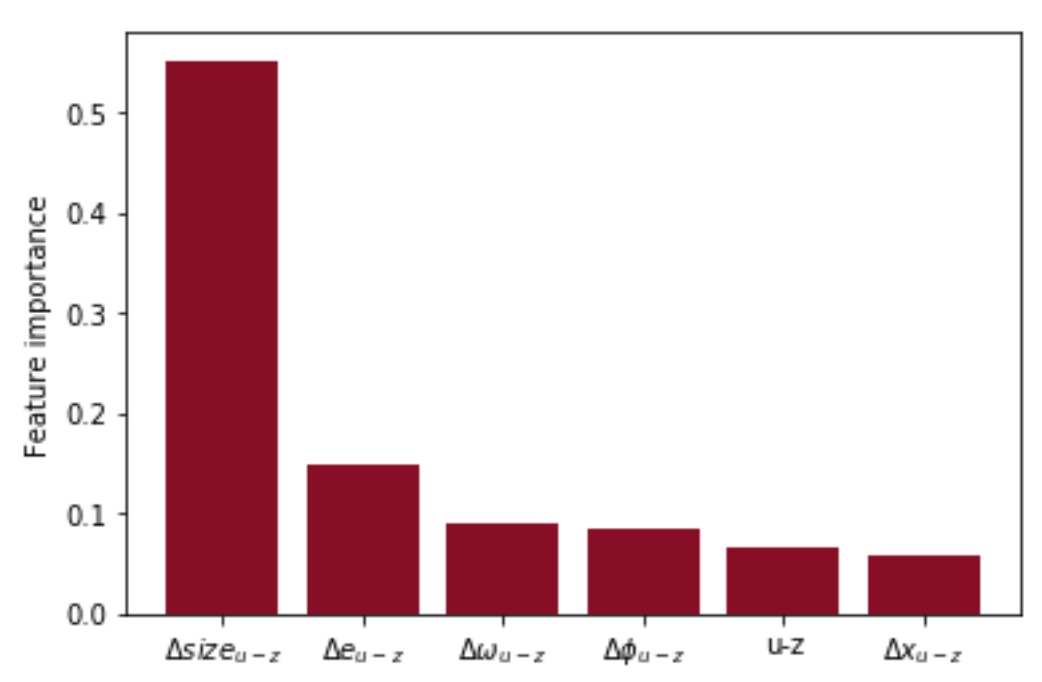
\includegraphics[width=0.4\columnwidth]{FeatureImportance.png}
\caption{Feature importance calculated with the Random Forest algorithm.}
 \label{fig:featureimportance}
\end{figure}

\subsection{Classification}
\label{subsec:classification_data}

As mentioned in \autoref{subsec:classification}, we used three different algorithms: linear SVC, KNeighbors (Nearest Neighbors), and
Random Forest. \autoref{fig:roc} shows the results that we got for
each algorithm.

Random forest showed the best performance among the three different
algorithms. If we look into the top left corner where all the curves are
overlapped, we can see this more obviously. The best classifiers were
Random Forest, and the more the number of estimators were, the better
the algorithm performed. For the best algorithm, we were able to achieve
~98$\%$ of the true positive rate(TPR) and ~0.04$\%$ of the false
positive rate(FPR).

\begin{figure}
    \centering
    \begin{minipage}{0.48\linewidth}        %% or \columnwidth
        \centering
        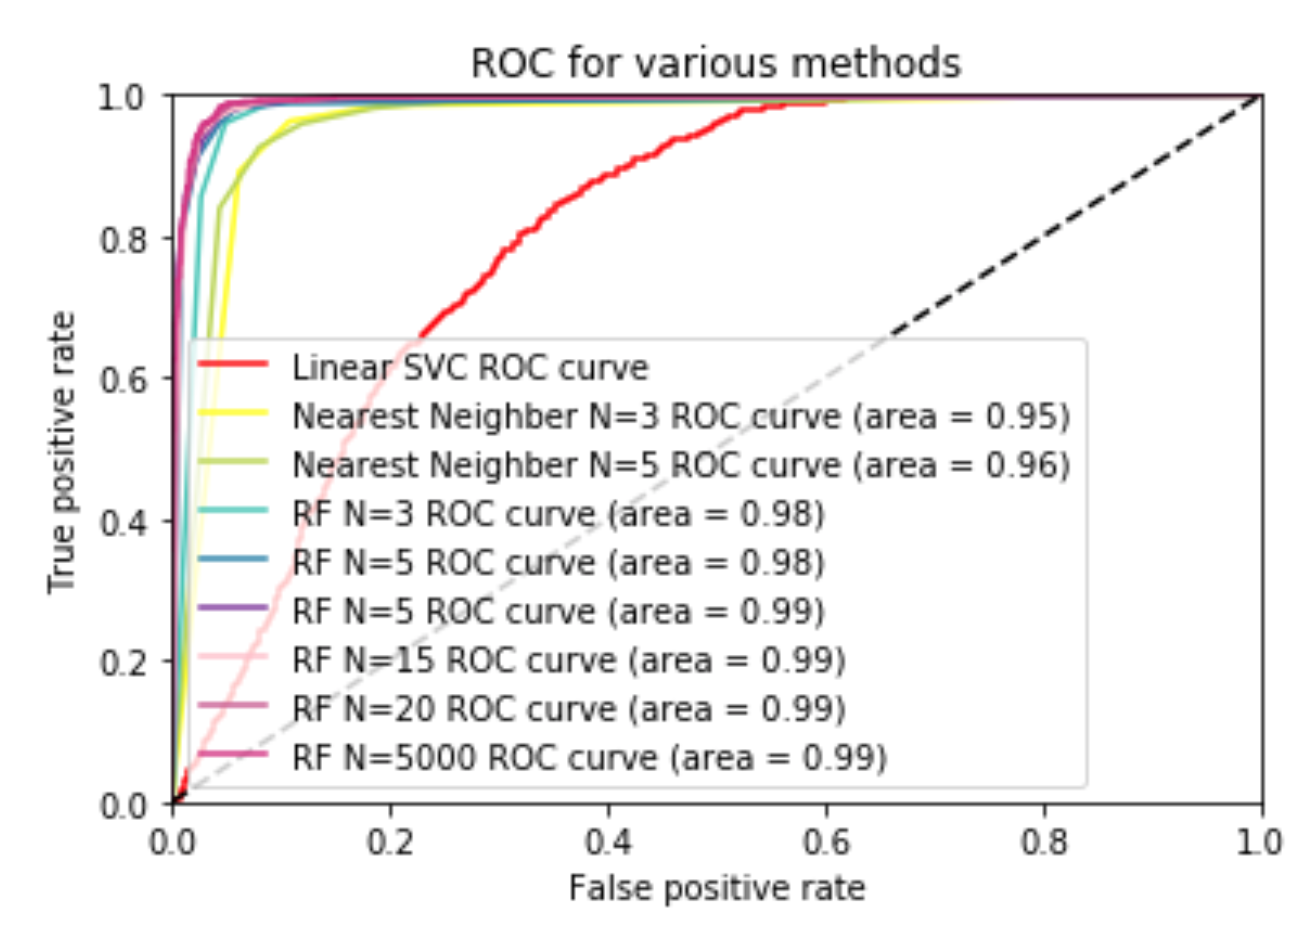
\includegraphics[width=\linewidth]{ML_notmagnified.png}
    \end{minipage}\hfill
    \begin{minipage}{0.48\linewidth}        %% or \columnwidth
        \centering
        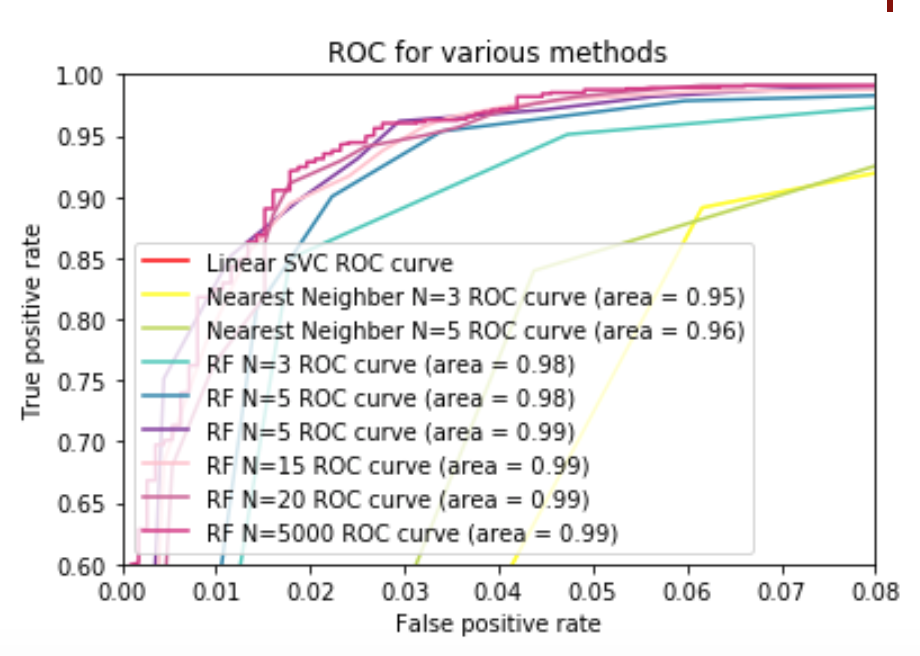
\includegraphics[width=\linewidth]{ML_magnified.png}
         \label{fig:ML Magnified}
    \end{minipage}
    \caption{ROC curves for lens-or-not machine classification on \SLRealizer-emulated LSST \Object data. Left: full view. Right: zoomed-in view over the axes ranges FPR=[0:0.08] and TPR=[0.6:1.0].}
    \label{fig:roc}
\end{figure}

% ----------------------------------------------------------------------

\section{Conclusions}
\label{sec:conclusions}

The results suggest that random forest algorithms would be able to
differentiate lensed systems from galaxies. Still, even though we have
high accuracy, because we expect to have much more non-lensed systems
than the lensed systems, we will have more contaminants in the
truly-classified lensed systems than the actual lensed systems. For
instance, we expect to find 10,000 times more non-lensed systems than
the lensed ones. Thus, with 98\% of the TPR and ~0.042\% of the FPR, we
will have ~430 contaminants per truly classified lensed systems. Thus,
it would also be helpful to have a more rigorous model that actually
fits physical models to the systems after rejecting all the non
lensed-systems using SLRealizer.

In addition, we only compared the features between OM10 lensed systems
and SDSS galaxies. It will also be useful to overlap star-star pairs,
star-galaxy pairs, quasar-quasar pairs, or quasar-galaxy pairs to see
how different the other samples could be from the lensed system.

There are few ways to further improve the classifiers. If we could
implement the working deblender that resembles LSST’s deblender, that
will increase the performance of the classifiers. We could also add more
features such as time-variabilities of quasar images. While making the
source and the object catalog, rather than giving equal weights to all
the observations, we could weight by how good the seeing was for each
night.

In addition, while studying cosmology, gravitationally lensed systems
with four images (quads) are generally more useful than the systems with
two images (doubles). Thus, comparing how many quads were classified as
true out of the testing sample’s quads should also give useful
statistics.

% ----------------------------------------------------------------------

\subsection*{Acknowledgments}

% 
This is the text imported from \code{acknowledgments.tex}, and will be replaced by some standard LSST DESC boilerplate at some point.
% 


Author contributions are listed below. \\
Jenny Kim: Initial algorithm and code development, wrote paper. \\
Ji Won Park: Improved algorithm and code development, edited paper. \\
Phil~Marshall: Initiated  project, advised on motivation, model construction and testing. \\
Mike~Baumer: Advised on LSST data characteristics, model construction and testing. \\
Steve~Kahn: Advised on LSST data characteristics, model construction and testing. \\
Rahul~Biswas: Advised on LSST observing cadence, catalog characteristics, error model. \\


%{\it Facilities:} \facility{LSST}
% Include both collaboration papers and external citations:
\bibliography{lsstdesc,main}

\end{document}
% ======================================================================
%
